\input{preamble.tex}

\title{Лабораторная работа № 1. \\ Знакомство с Cisco Packet Tracer}
\author{Сущенко Алина \\ НПИбд-01-23}

\institute{Российский университет дружбы народов имени Патриса Лумумбы}
\date{2026}

\begin{document}

\frame{\titlepage}

\begin{frame}
\frametitle{Цель работы}
\begin{itemize}
    \item Установить инструмент моделирования конфигурации сети \texttt{Cisco Packet Tracer}.
    \item Ознакомиться с интерфейсом программы.
    \item Изучить принципы работы концентратора, коммутатора и маршрутизатора.
    \item Исследовать протоколы ARP, ICMP, STP, CDP.
\end{itemize}
\end{frame}

\begin{frame}
\frametitle{Запуск Cisco Packet Tracer без использования сетевого соединения}
    \centering
    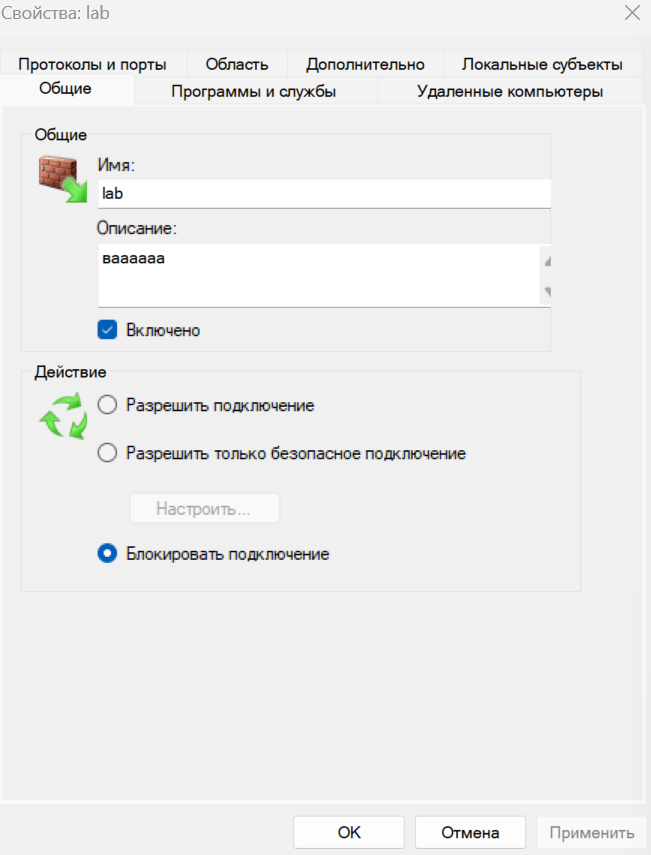
\includegraphics[width=0.8\textwidth]{../images/01.png}
    \captionof{figure}{Конечная настройка подключения к сети (часть с ограничением подключения).}
\end{frame}

\begin{frame}
\frametitle{Запуск Cisco Packet Tracer без использования сетевого соединения}
    \centering
    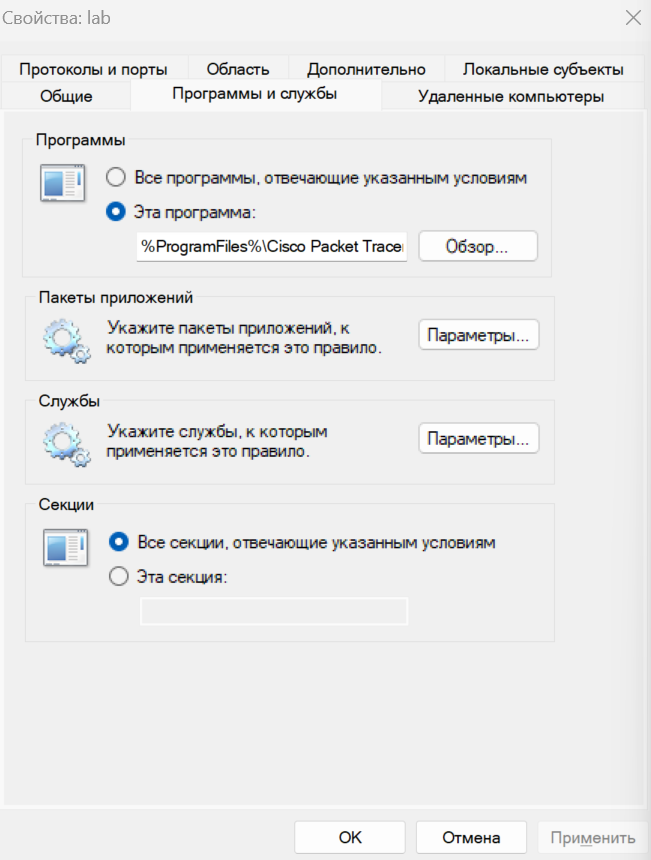
\includegraphics[width=0.8\textwidth]{../images/02.png}
    \captionof{figure}{Конечная настройка подключения к сети (часть с расположением файла на компьютере).}
\end{frame}

\begin{frame}
\frametitle{Знакомство с интерфейсом Packet Tracer}
    \centering
    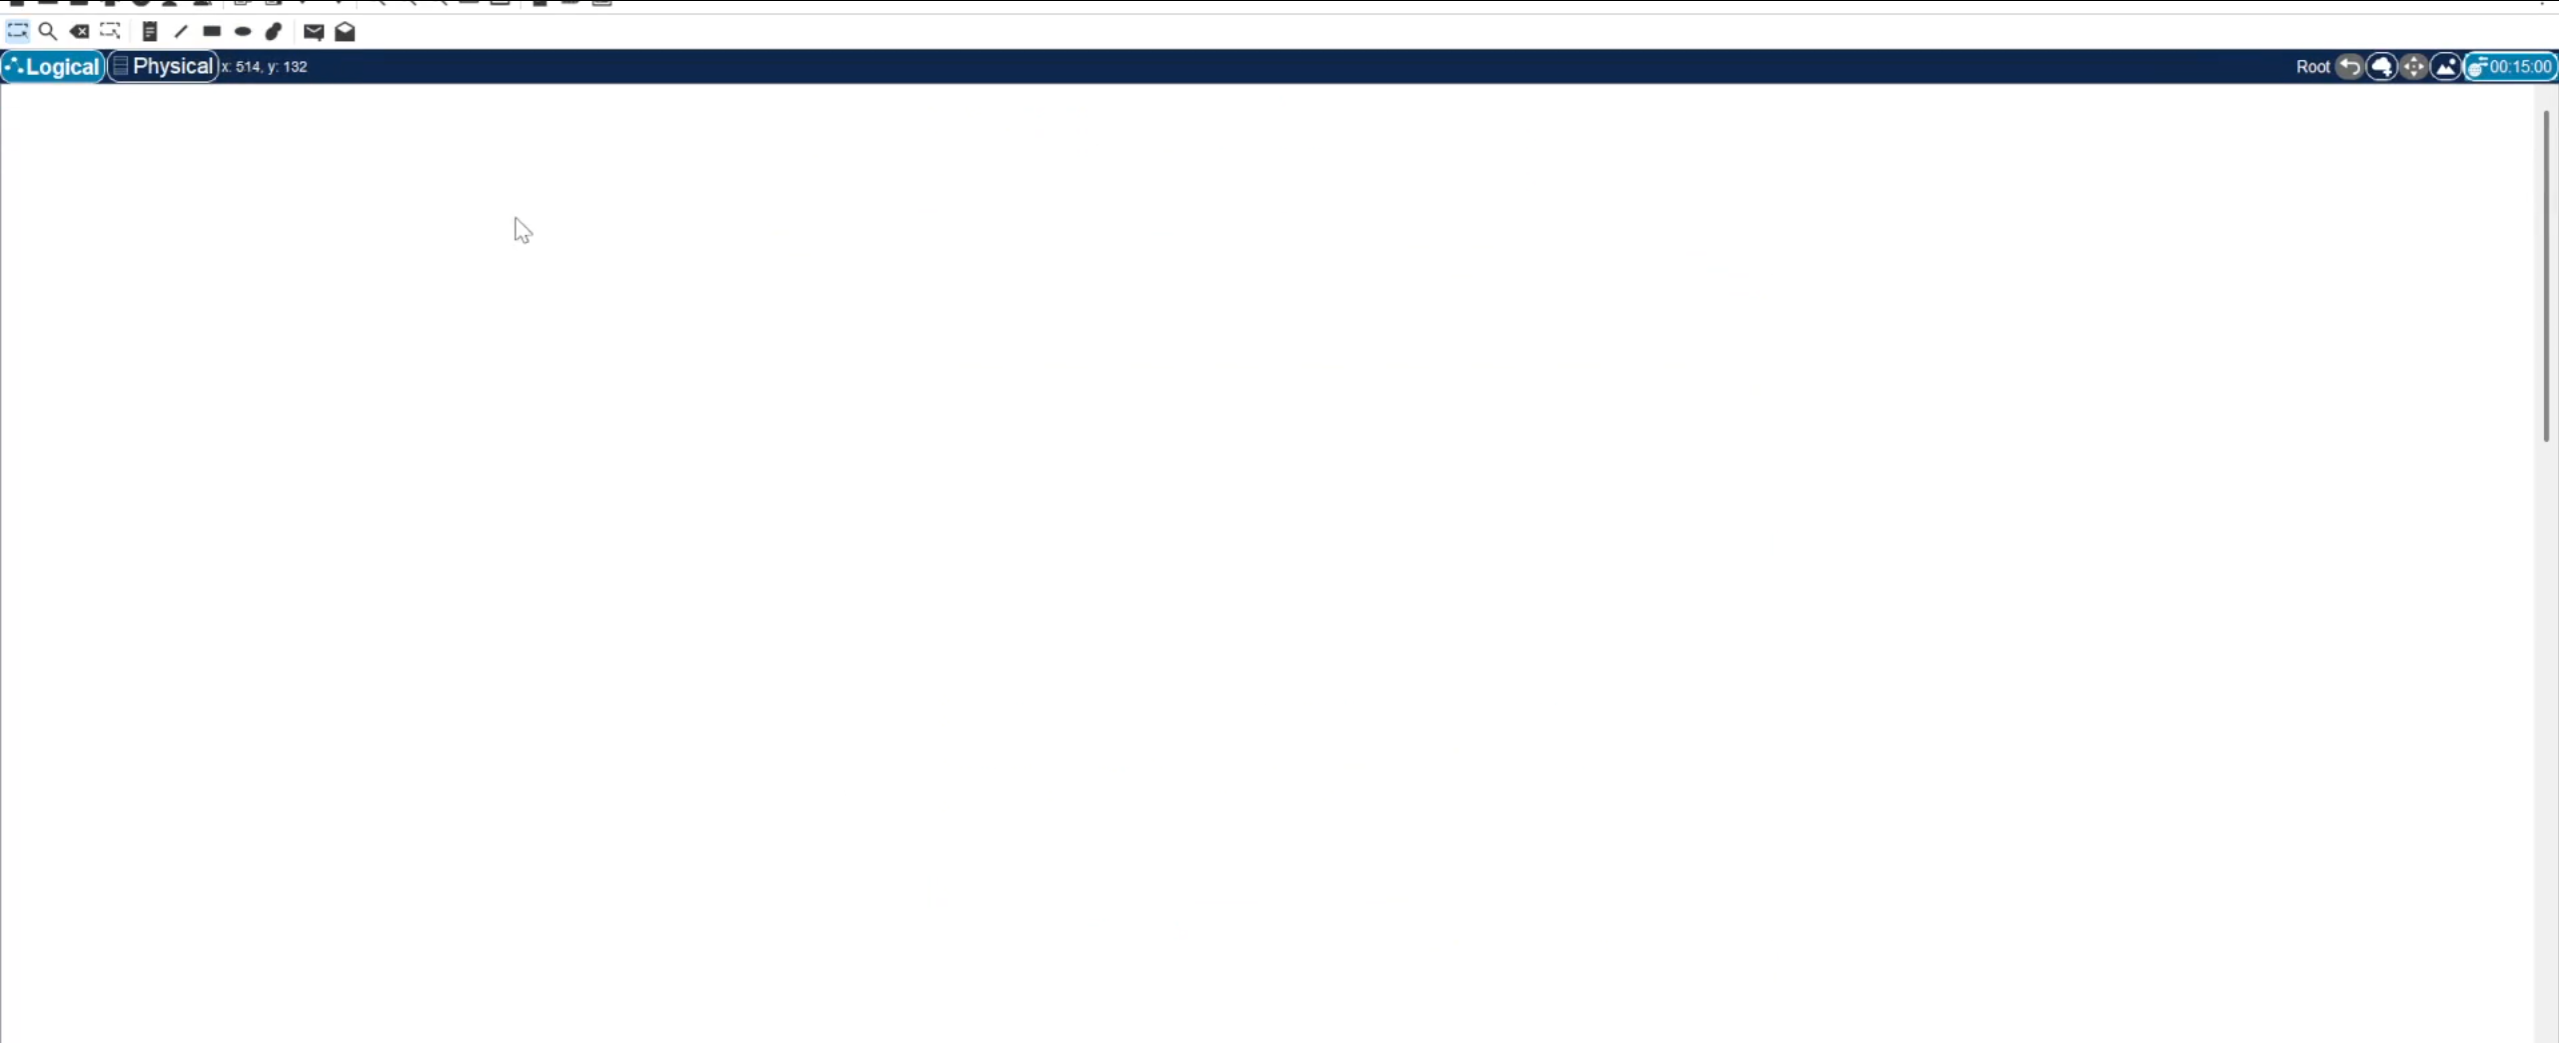
\includegraphics[width=0.8\textwidth]{../images/03.png}
    \captionof{figure}{Чистое рабочее пространство.}
\end{frame}

\begin{frame}
\frametitle{Построение простейшей сети с концентратором}
    \centering
    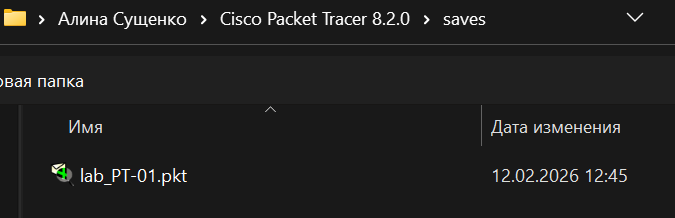
\includegraphics[width=0.8\textwidth]{../images/04.png}
    \captionof{figure}{Созданный проект lab\_PT-01.pkt.}
\end{frame}

\begin{frame}
\frametitle{Построение простейшей сети с концентратором}
    \centering
    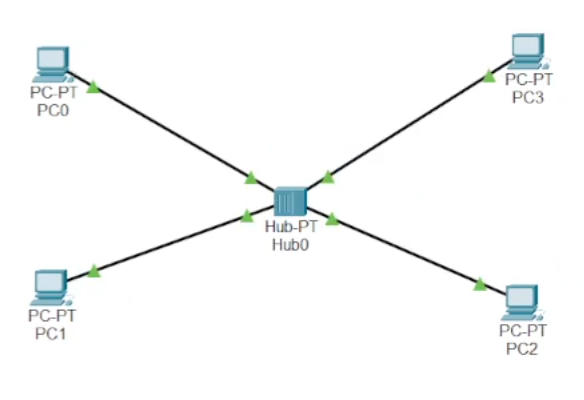
\includegraphics[width=0.8\textwidth]{../images/05.png}
    \captionof{figure}{Модель простой сети с концентратором.}
\end{frame}

\begin{frame}
\frametitle{Настройка IP-адресов на устройствах}
    \centering
    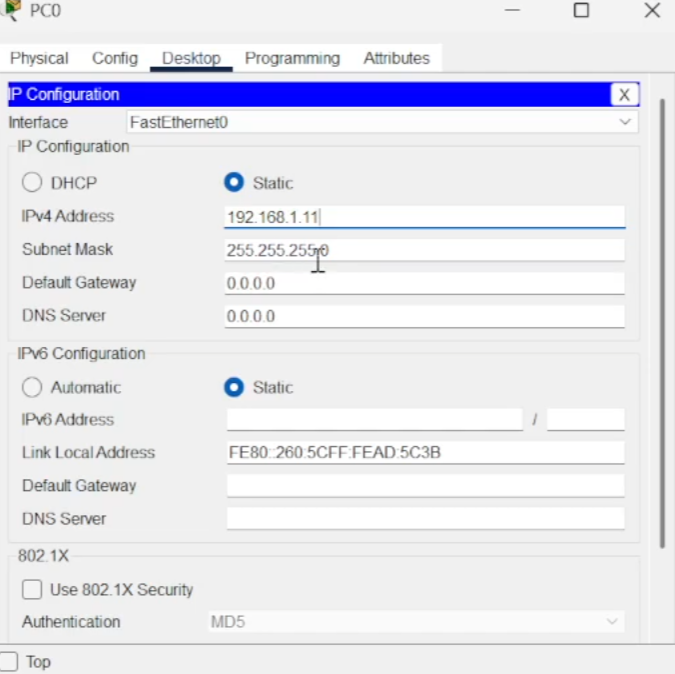
\includegraphics[width=0.45\textwidth]{../images/06.png}
    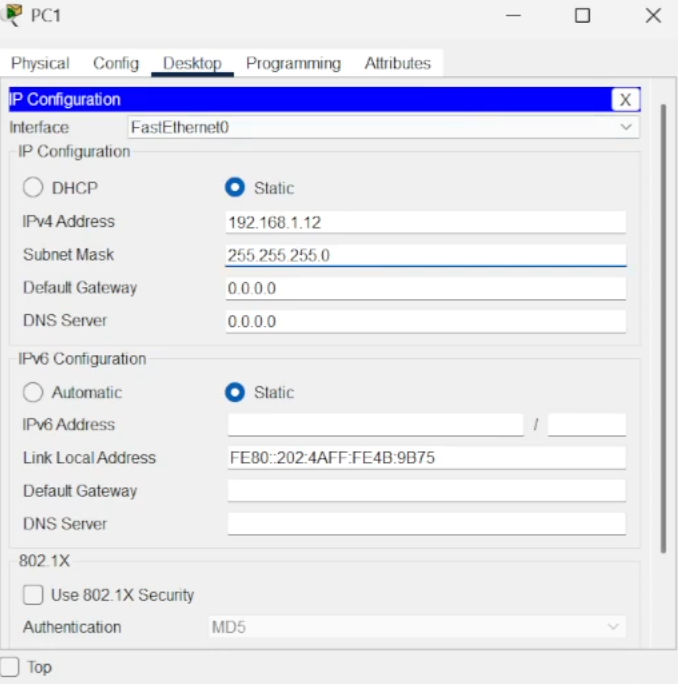
\includegraphics[width=0.45\textwidth]{../images/07.png}
    \captionof{figure}{Статические IP-адреса для PC0 и PC1.}
\end{frame}

\begin{frame}
\frametitle{Настройка IP-адресов на устройствах}
    \centering
    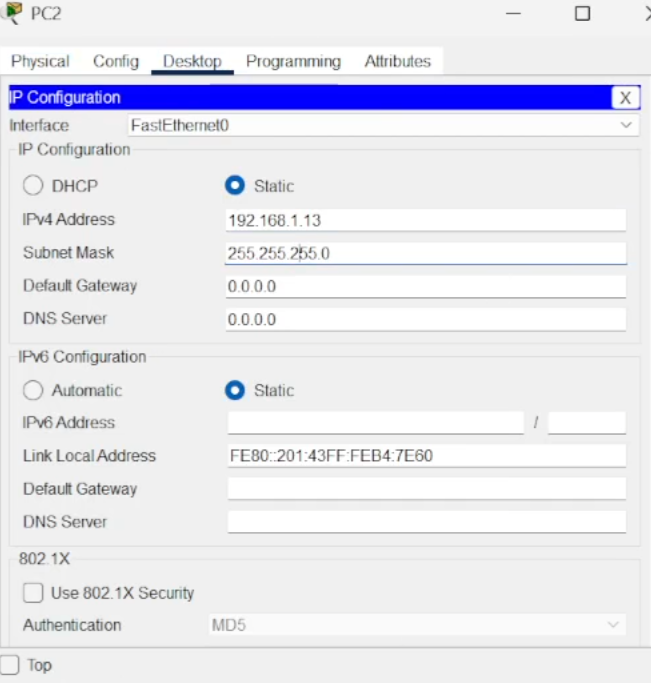
\includegraphics[width=0.45\textwidth]{../images/08.png}
    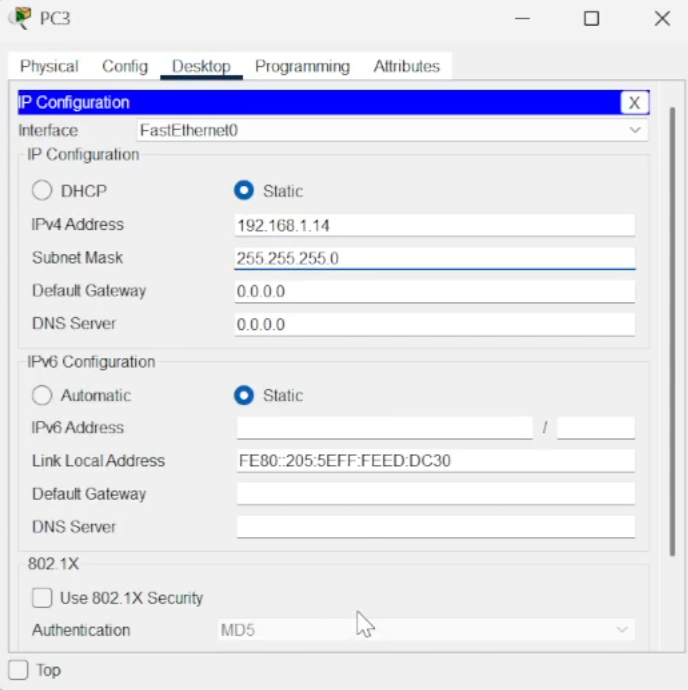
\includegraphics[width=0.45\textwidth]{../images/09.png}
    \captionof{figure}{Статические IP-адреса для PC2 и PC3.}
\end{frame}

\begin{frame}
\frametitle{Моделирование передачи пакетов ARP и ICMP}
    \centering
    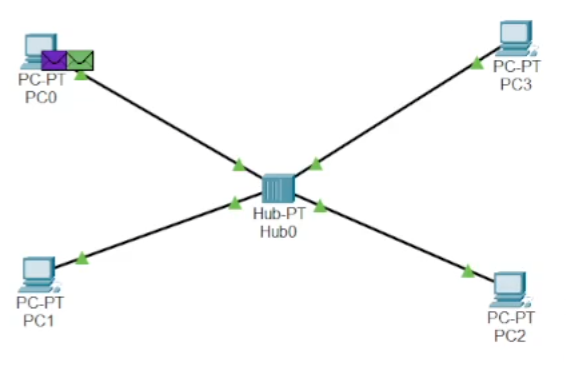
\includegraphics[width=0.8\textwidth]{../images/10.png}
    \captionof{figure}{Два конверта в рабочей области.}
\end{frame}

\begin{frame}
\frametitle{Моделирование передачи пакетов ARP и ICMP}
    \centering
    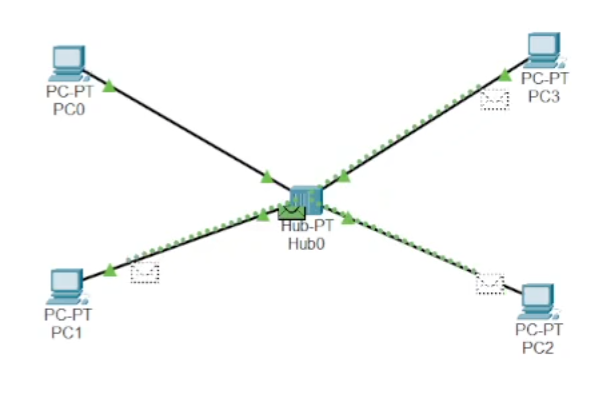
\includegraphics[width=0.8\textwidth]{../images/11.png}
    \captionof{figure}{Движение конвертов.}
\end{frame}

\begin{frame}
\frametitle{Исследование PDU и модели OSI}
    \centering
    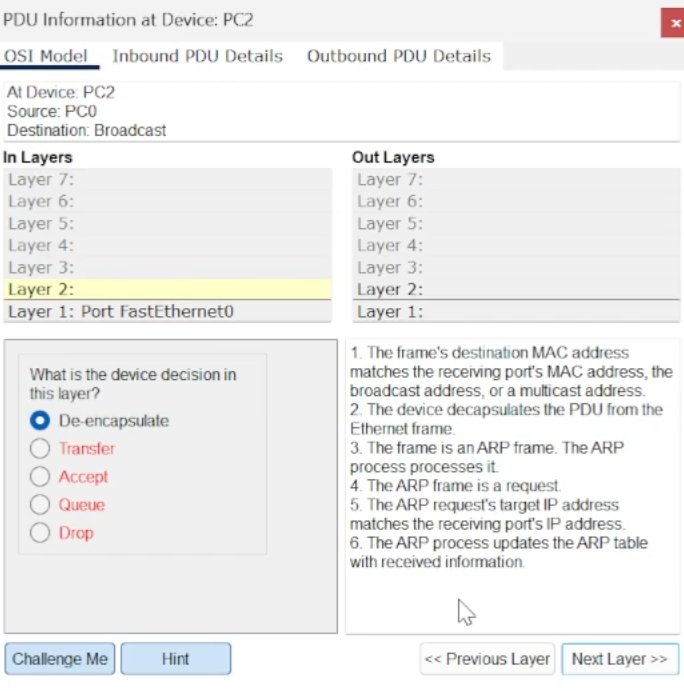
\includegraphics[width=0.8\textwidth]{../images/12.png}
    \captionof{figure}{Вкладка OSI Model и Challenge Me.}
\end{frame}

\begin{frame}
\frametitle{Исследование PDU и модели OSI}
    \centering
    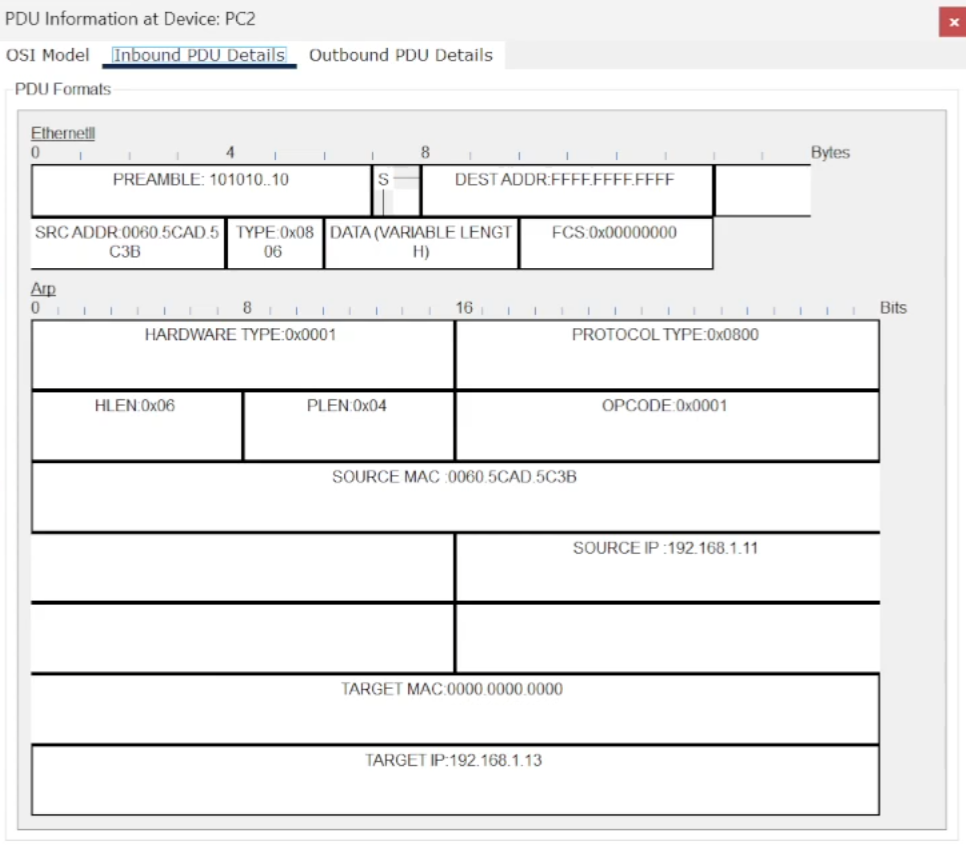
\includegraphics[width=0.8\textwidth]{../images/13.png}
    \captionof{figure}{Вкладка информации о PDU.}
\end{frame}

\begin{frame}
\frametitle{Возникновение коллизии в сети с концентратором}
    \centering
    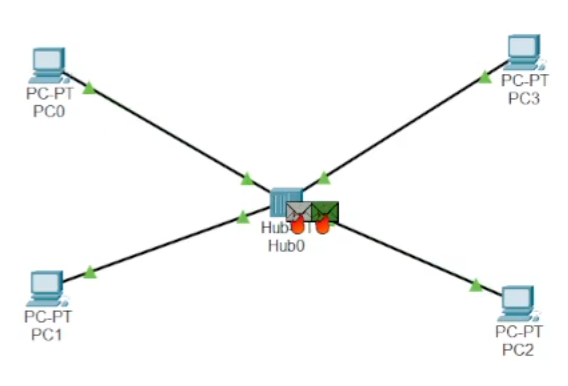
\includegraphics[width=0.8\textwidth]{../images/14.png}
    \captionof{figure}{Коллизия при одновременной передаче.}
\end{frame}

\begin{frame}
\frametitle{Построение сети с коммутатором}
    \centering
    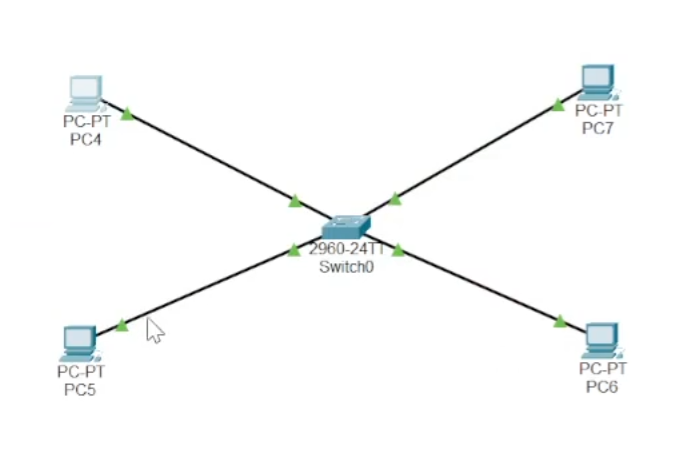
\includegraphics[width=0.8\textwidth]{../images/15.png}
    \captionof{figure}{Модель простой сети с коммутатором.}
\end{frame}

\begin{frame}
\frametitle{Настройка IP-адресов на устройствах}
    \centering
    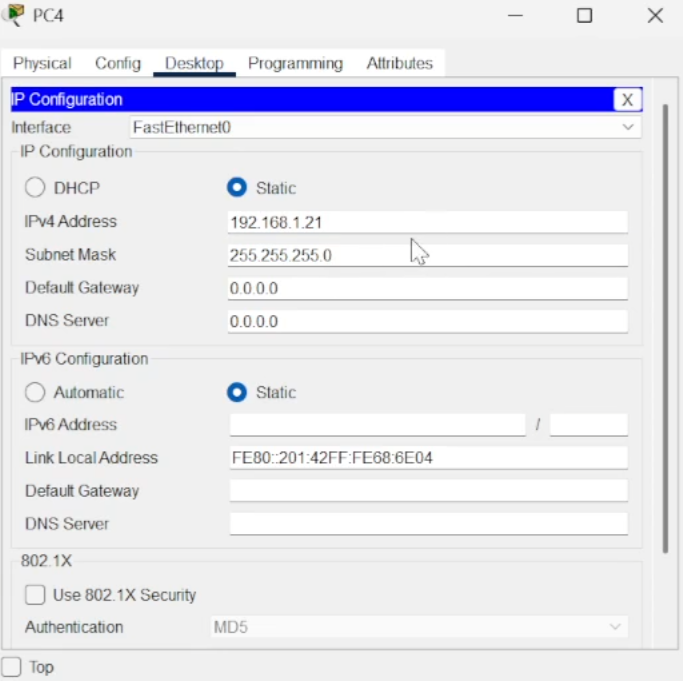
\includegraphics[width=0.45\textwidth]{../images/16.png}
    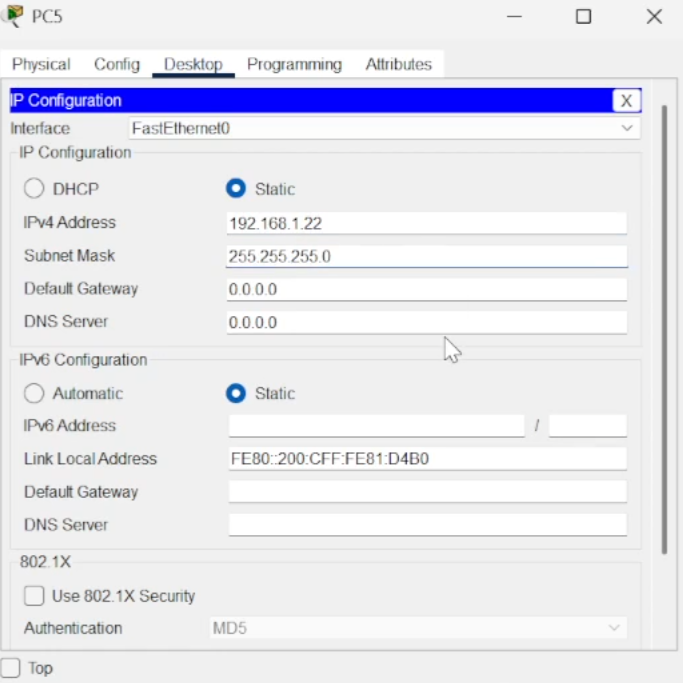
\includegraphics[width=0.45\textwidth]{../images/17.png}
    \captionof{figure}{Статические IP-адреса для PC4 и PC5.}
\end{frame}

\begin{frame}
\frametitle{Настройка IP-адресов на устройствах}
    \centering
    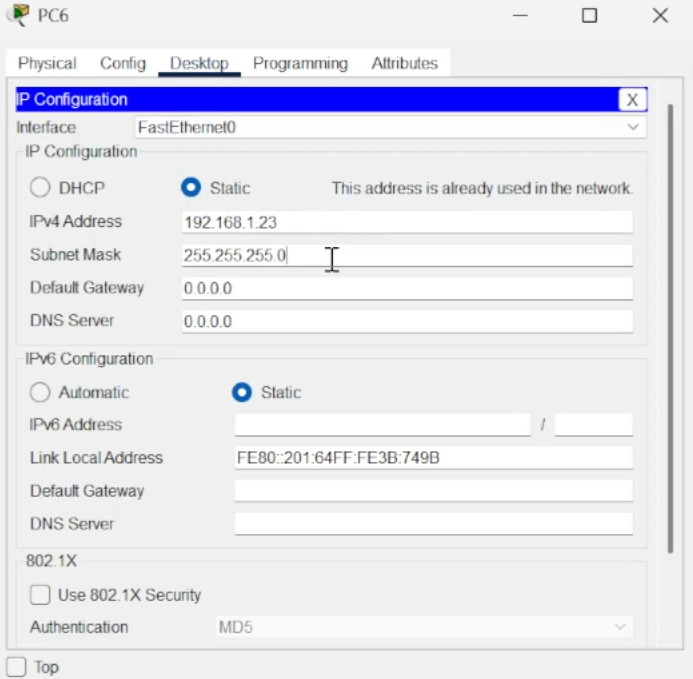
\includegraphics[width=0.45\textwidth]{../images/18.png}
    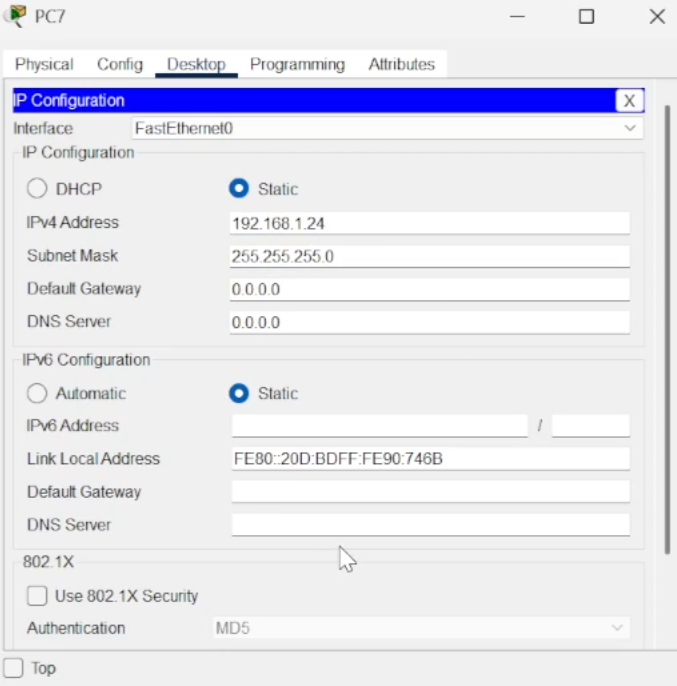
\includegraphics[width=0.45\textwidth]{../images/19.png}
    \captionof{figure}{Статические IP-адреса для PC6 и PC7.}
\end{frame}

\begin{frame}
\frametitle{Моделирование передачи пакетов с коммутатором}
    \centering
    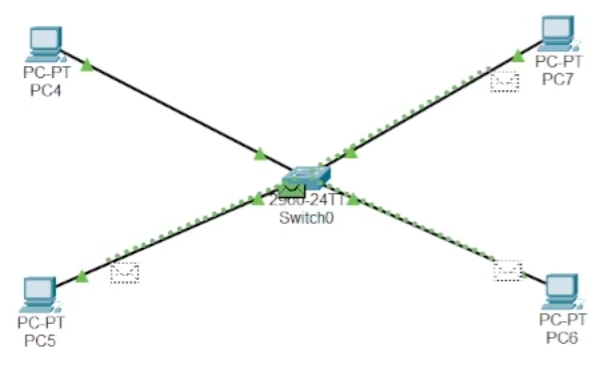
\includegraphics[width=0.8\textwidth]{../images/20.png}
    \captionof{figure}{Движение пакетов ARP и ICMP в сети с коммутатором.}
\end{frame}

\begin{frame}
\frametitle{Отсутствие коллизии в сети с коммутатором}
    \centering
    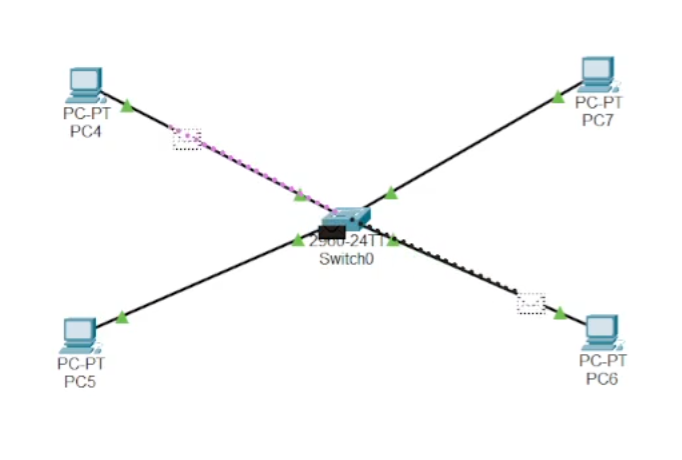
\includegraphics[width=0.8\textwidth]{../images/21.png}
    \captionof{figure}{Отсутствие коллизии при одновременной передаче.}
\end{frame}

\begin{frame}
\frametitle{Соединение концентратора и коммутатора}
    \centering
    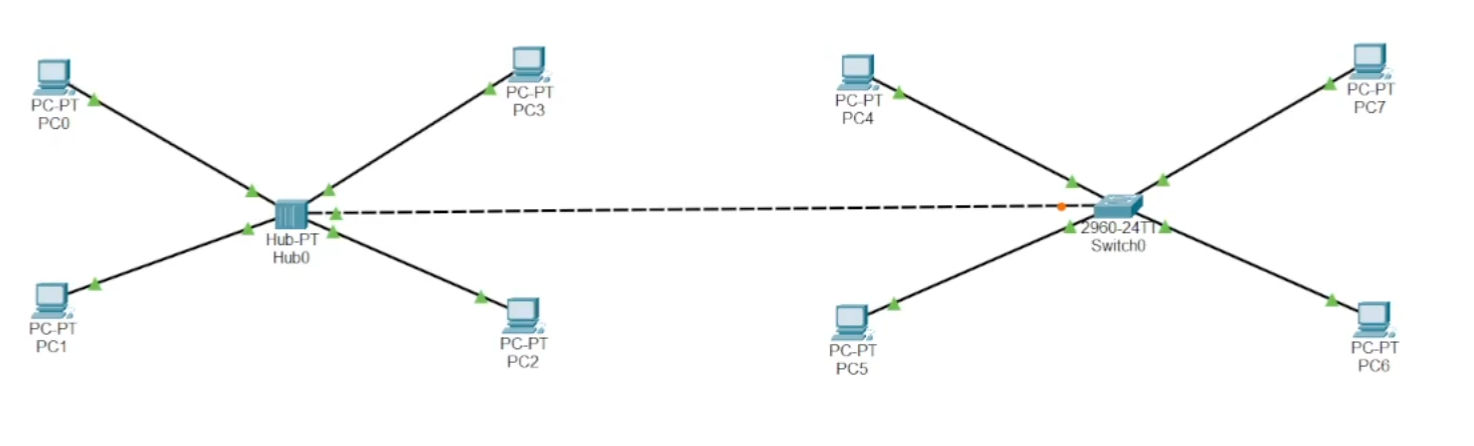
\includegraphics[width=0.8\textwidth]{../images/22.png}
    \captionof{figure}{Соединение двух схем кроссовым кабелем.}
\end{frame}

\begin{frame}
\frametitle{Возникновение коллизии в гибридной сети}
    \centering
    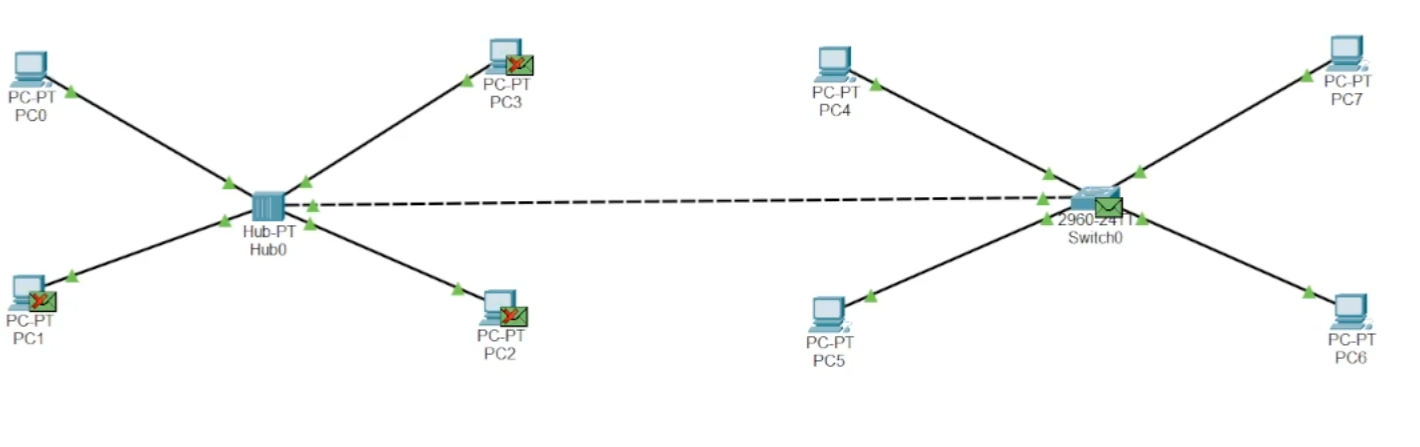
\includegraphics[width=0.8\textwidth]{../images/23.png}
    \captionof{figure}{Коллизия при передаче через концентратор и коммутатор.}
\end{frame}

\begin{frame}
\frametitle{Исследование STP (Spanning Tree Protocol)}
    \centering
    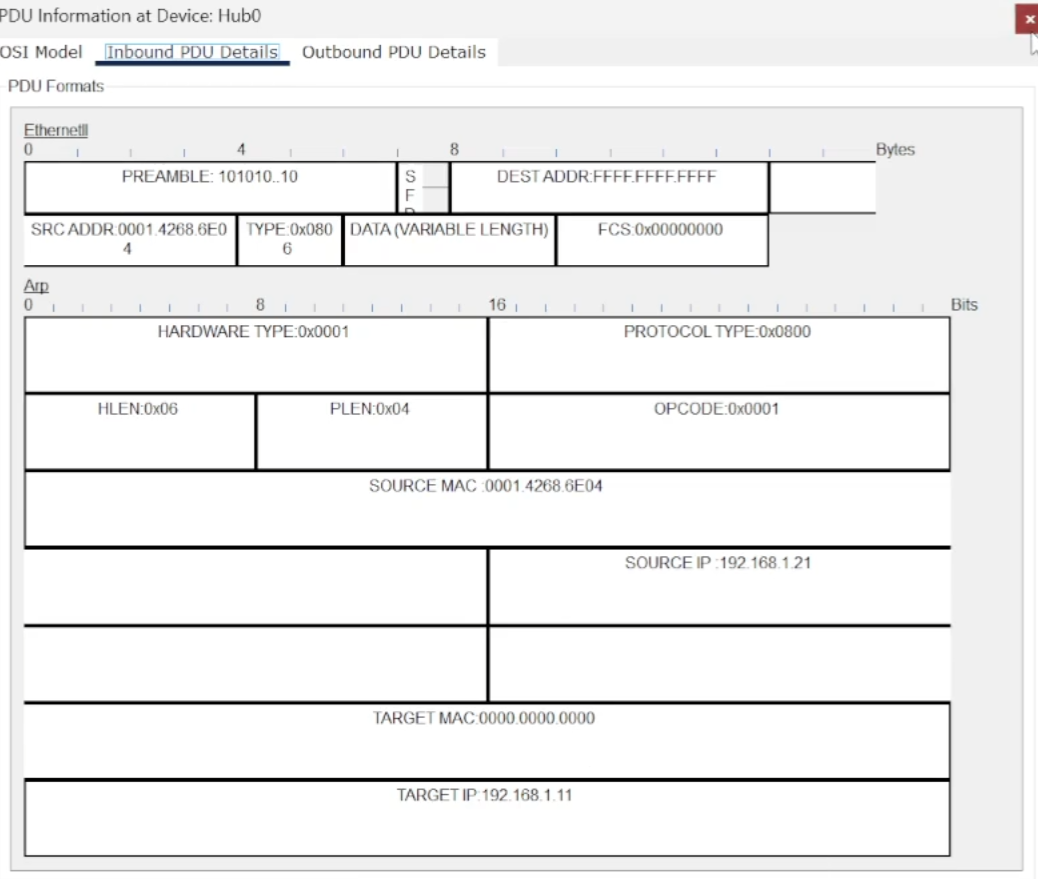
\includegraphics[width=0.8\textwidth]{../images/24.png}
    \captionof{figure}{Пакеты STP (BPDU) в списке событий.}
\end{frame}

\begin{frame}
\frametitle{Добавление маршрутизатора}
    \centering
    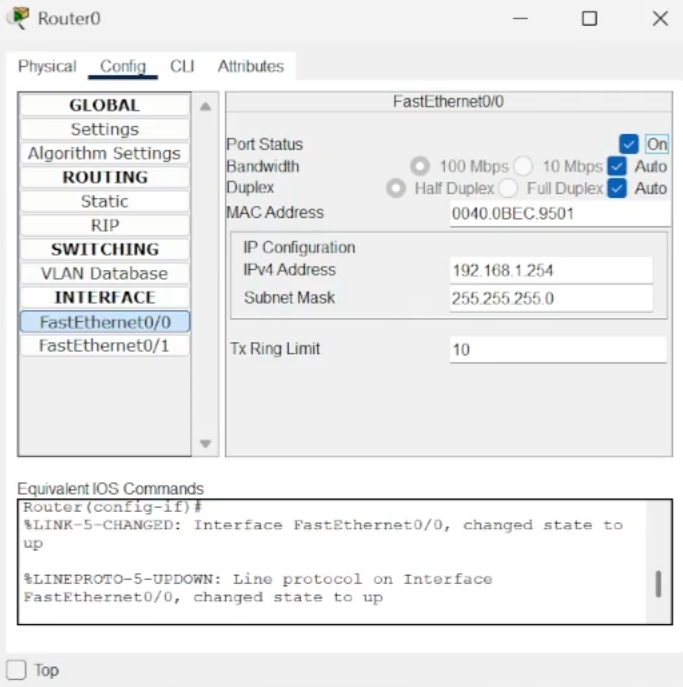
\includegraphics[width=0.8\textwidth]{../images/25.png}
    \captionof{figure}{Настройка IP-адреса на маршрутизаторе.}
\end{frame}

\begin{frame}
\frametitle{Структура кадра Ethernet для различных протоколов}

\begin{tabular}{|l|l|l|}
\hline
\textbf{Протокол} & \textbf{Тип кадра} & \textbf{Destination MAC} \\
\hline
STP (BPDU) & 802.3 + LLC & 01:80:C2:00:00:00 \\
CDP & Ethernet II & 01:00:0C:CC:CC:CC \\
ARP & Ethernet II & FF:FF:FF:FF:FF:FF \\
ICMP (IPv4) & Ethernet II & MAC получателя \\
\hline
\end{tabular}

\vspace{0.5cm}
\textbf{Структура ICMP-пакета:}
\begin{tabular}{|l|c|}
\hline
\textbf{Поле} & \textbf{Длина} \\
\hline
Type & 1 байт \\
Code & 1 байт \\
Checksum & 2 байта \\
Identifier & 2 байта \\
Sequence Number & 2 байта \\
Data & переменная \\
\hline
\end{tabular}
\end{frame}

\subsection*{Контрольные вопросы}

\begin{frame}
\frametitle{Контрольные вопросы}

\begin{block}{1. Дайте определение следующим понятиям: концентратор, коммутатор, маршрутизатор, шлюз (gateway). В каких случаях следует использовать тот или иной тип сетевого оборудования?}
\textbf{Концентратор (Hub)} - устройство физического уровня (L1), которое ретранслирует входящие сигналы на все порты, кроме входящего. Не анализирует трафик, не буферизирует кадры. Используется в небольших сетях, где допустимы коллизии и низкая производительность.

\textbf{Коммутатор (Switch)} - устройство канального уровня (L2), которое анализирует MAC-адреса, строит CAM-таблицу и передаёт кадры адресно на целевой порт. Используется для сегментации сети, разделения доменов коллизий, повышения производительности.

\textbf{Маршрутизатор (Router)} - устройство сетевого уровня (L3), которое обеспечивает связь между различными IP-подсетями, выполняет маршрутизацию на основе IP-адресов, изменяет MAC-адреса при передаче. Используется для объединения сетей, обеспечения безопасности, NAT.

\textbf{Шлюз (Gateway)} - узел сети, который обеспечивает доступ в другие сети (обычно маршрутизатор). Используется как точка выхода в другую подсеть или Интернет.
\end{block}
\end{frame}

\begin{frame}
\frametitle{Контрольные вопросы}

\begin{block}{2. Дайте определение следующим понятиям: ip-адрес, сетевая маска, broadcast-адрес.}
\textbf{IP-адрес} - уникальный идентификатор устройства в сети, работающий на сетевом уровне. Состоит из 32 бит (IPv4), записывается в виде четырёх десятичных чисел, разделённых точками (например, 192.168.1.11).

\textbf{Сетевая маска (Subnet Mask)} - 32-битное число, которое определяет, какая часть IP-адреса относится к адресу сети, а какая - к адресу узла. Записывается аналогично IP-адресу (например, 255.255.255.0).

\textbf{Broadcast-адрес} - специальный адрес, который используется для отправки пакетов всем узлам в данной подсети. Формируется путём установки всех битов узла в 1 (например, 192.168.1.255 для сети 192.168.1.0/24).
\end{block}
\end{frame}

\begin{frame}
\frametitle{Контрольные вопросы}

\begin{block}{3. Как можно проверить доступность узла сети?}
Основные способы проверки доступности узла:

\begin{itemize}
\item \textbf{ping} - отправка ICMP Echo Request и получение ICMP Echo Reply. Проверяет доступность узла на сетевом уровне.
\item \textbf{traceroute / tracert} - отслеживание маршрута следования пакетов до узла назначения.
\item \textbf{arp} - просмотр ARP-таблицы для проверки соответствия IP- и MAC-адресов.
\item \textbf{telnet / ssh} - проверка доступности определённого порта на узле.
\item \textbf{nslookup / dig} - проверка разрешения доменных имён в IP-адреса.
\end{itemize}

В Packet Tracer дополнительно можно использовать:
\begin{itemize}
\item \textbf{Add Simple PDU} - отправка тестового пакета между устройствами.
\item \textbf{Simulation mode} - пошаговый анализ передачи пакетов.
\end{itemize}
\end{block}
\end{frame}

\begin{frame}
\frametitle{Выводы}
\begin{itemize}
    \item Установили и настроили Cisco Packet Tracer для работы без сетевого соединения.
    \item Построили сети с концентратором, коммутатором и маршрутизатором.
    \item Настроили статическую IP-адресацию на оконечных устройствах.
    \item Исследовали поведение протоколов ARP, ICMP, STP и CDP.
    \item Изучили структуру кадров Ethernet и пакетов различных протоколов.
    \item Проанализировали возникновение коллизий в сетях с концентратором и их отсутствие в сетях с коммутатором.
    \item Изучили принципы работы STP для предотвращения петель в сети.
    \item Исследовали проприетарный протокол Cisco CDP для обнаружения соседних устройств.
    \item Получили практические навыки работы в режимах Realtime и Simulation.
\end{itemize}
\end{frame}

\end{document}
